\documentclass[11pt,a4paper]{report}
\usepackage[textwidth=37em,vmargin=30mm]{geometry}
\usepackage{calc,xunicode,amsmath,amssymb,paralist,enumitem,tabu,booktabs,datetime2,xeCJK,xeCJKfntef,listings}
\usepackage{tocloft,fancyhdr,tcolorbox,xcolor,graphicx,eso-pic,xltxtra,xelatexemoji}

\newcommand{\envyear}[0]{2025}
\newcommand{\envdatestr}[0]{2025-09-18}
\newcommand{\envfinaldir}[0]{webdb/2025/20250918/final}

\usepackage[hidelinks]{hyperref}
\hypersetup{
    colorlinks=false,
    pdfpagemode=FullScreen,
    pdftitle={Web Digest - \envdatestr}
}

\setlength{\cftbeforechapskip}{10pt}
\renewcommand{\cftchapfont}{\rmfamily\bfseries\large\raggedright}
\setlength{\cftbeforesecskip}{2pt}
\renewcommand{\cftsecfont}{\sffamily\small\raggedright}

\setdefaultleftmargin{2em}{2em}{1em}{1em}{1em}{1em}

\usepackage{xeCJK,xeCJKfntef}
\xeCJKsetup{PunctStyle=plain,RubberPunctSkip=false,CJKglue=\strut\hskip 0pt plus 0.1em minus 0.05em,CJKecglue=\strut\hskip 0.22em plus 0.2em}
\XeTeXlinebreaklocale "zh"
\XeTeXlinebreakskip = 0pt


\setmainfont{Brygada 1918}
\setromanfont{Brygada 1918}
\setsansfont{IBM Plex Sans}
\setmonofont{JetBrains Mono NL}
\setCJKmainfont{Noto Serif CJK SC}
\setCJKromanfont{Noto Serif CJK SC}
\setCJKsansfont{Noto Sans CJK SC}
\setCJKmonofont{Noto Sans CJK SC}

\setlength{\parindent}{0pt}
\setlength{\parskip}{8pt}
\linespread{1.15}

\lstset{
	basicstyle=\ttfamily\footnotesize,
	numbersep=5pt,
	backgroundcolor=\color{black!5},
	showspaces=false,
	showstringspaces=false,
	showtabs=false,
	tabsize=2,
	captionpos=b,
	breaklines=true,
	breakatwhitespace=true,
	breakautoindent=true,
	linewidth=\textwidth
}






\newcommand{\coverpic}[2]{
    % argv: itemurl, authorname
    Cover photo by #2~~(\href{#1}{#1})
}
\newcommand{\makeheader}[0]{
    \begin{titlepage}
        % \newgeometry{hmargin=15mm,tmargin=21mm,bmargin=12mm}
        \begin{center}
            
            \rmfamily\scshape
            \fontspec{BaskervilleF}
            \fontspec{Old Standard}
            \fontsize{59pt}{70pt}\selectfont
            WEB\hfill DIGEST
            
            \vfill
            % \vskip 30pt
            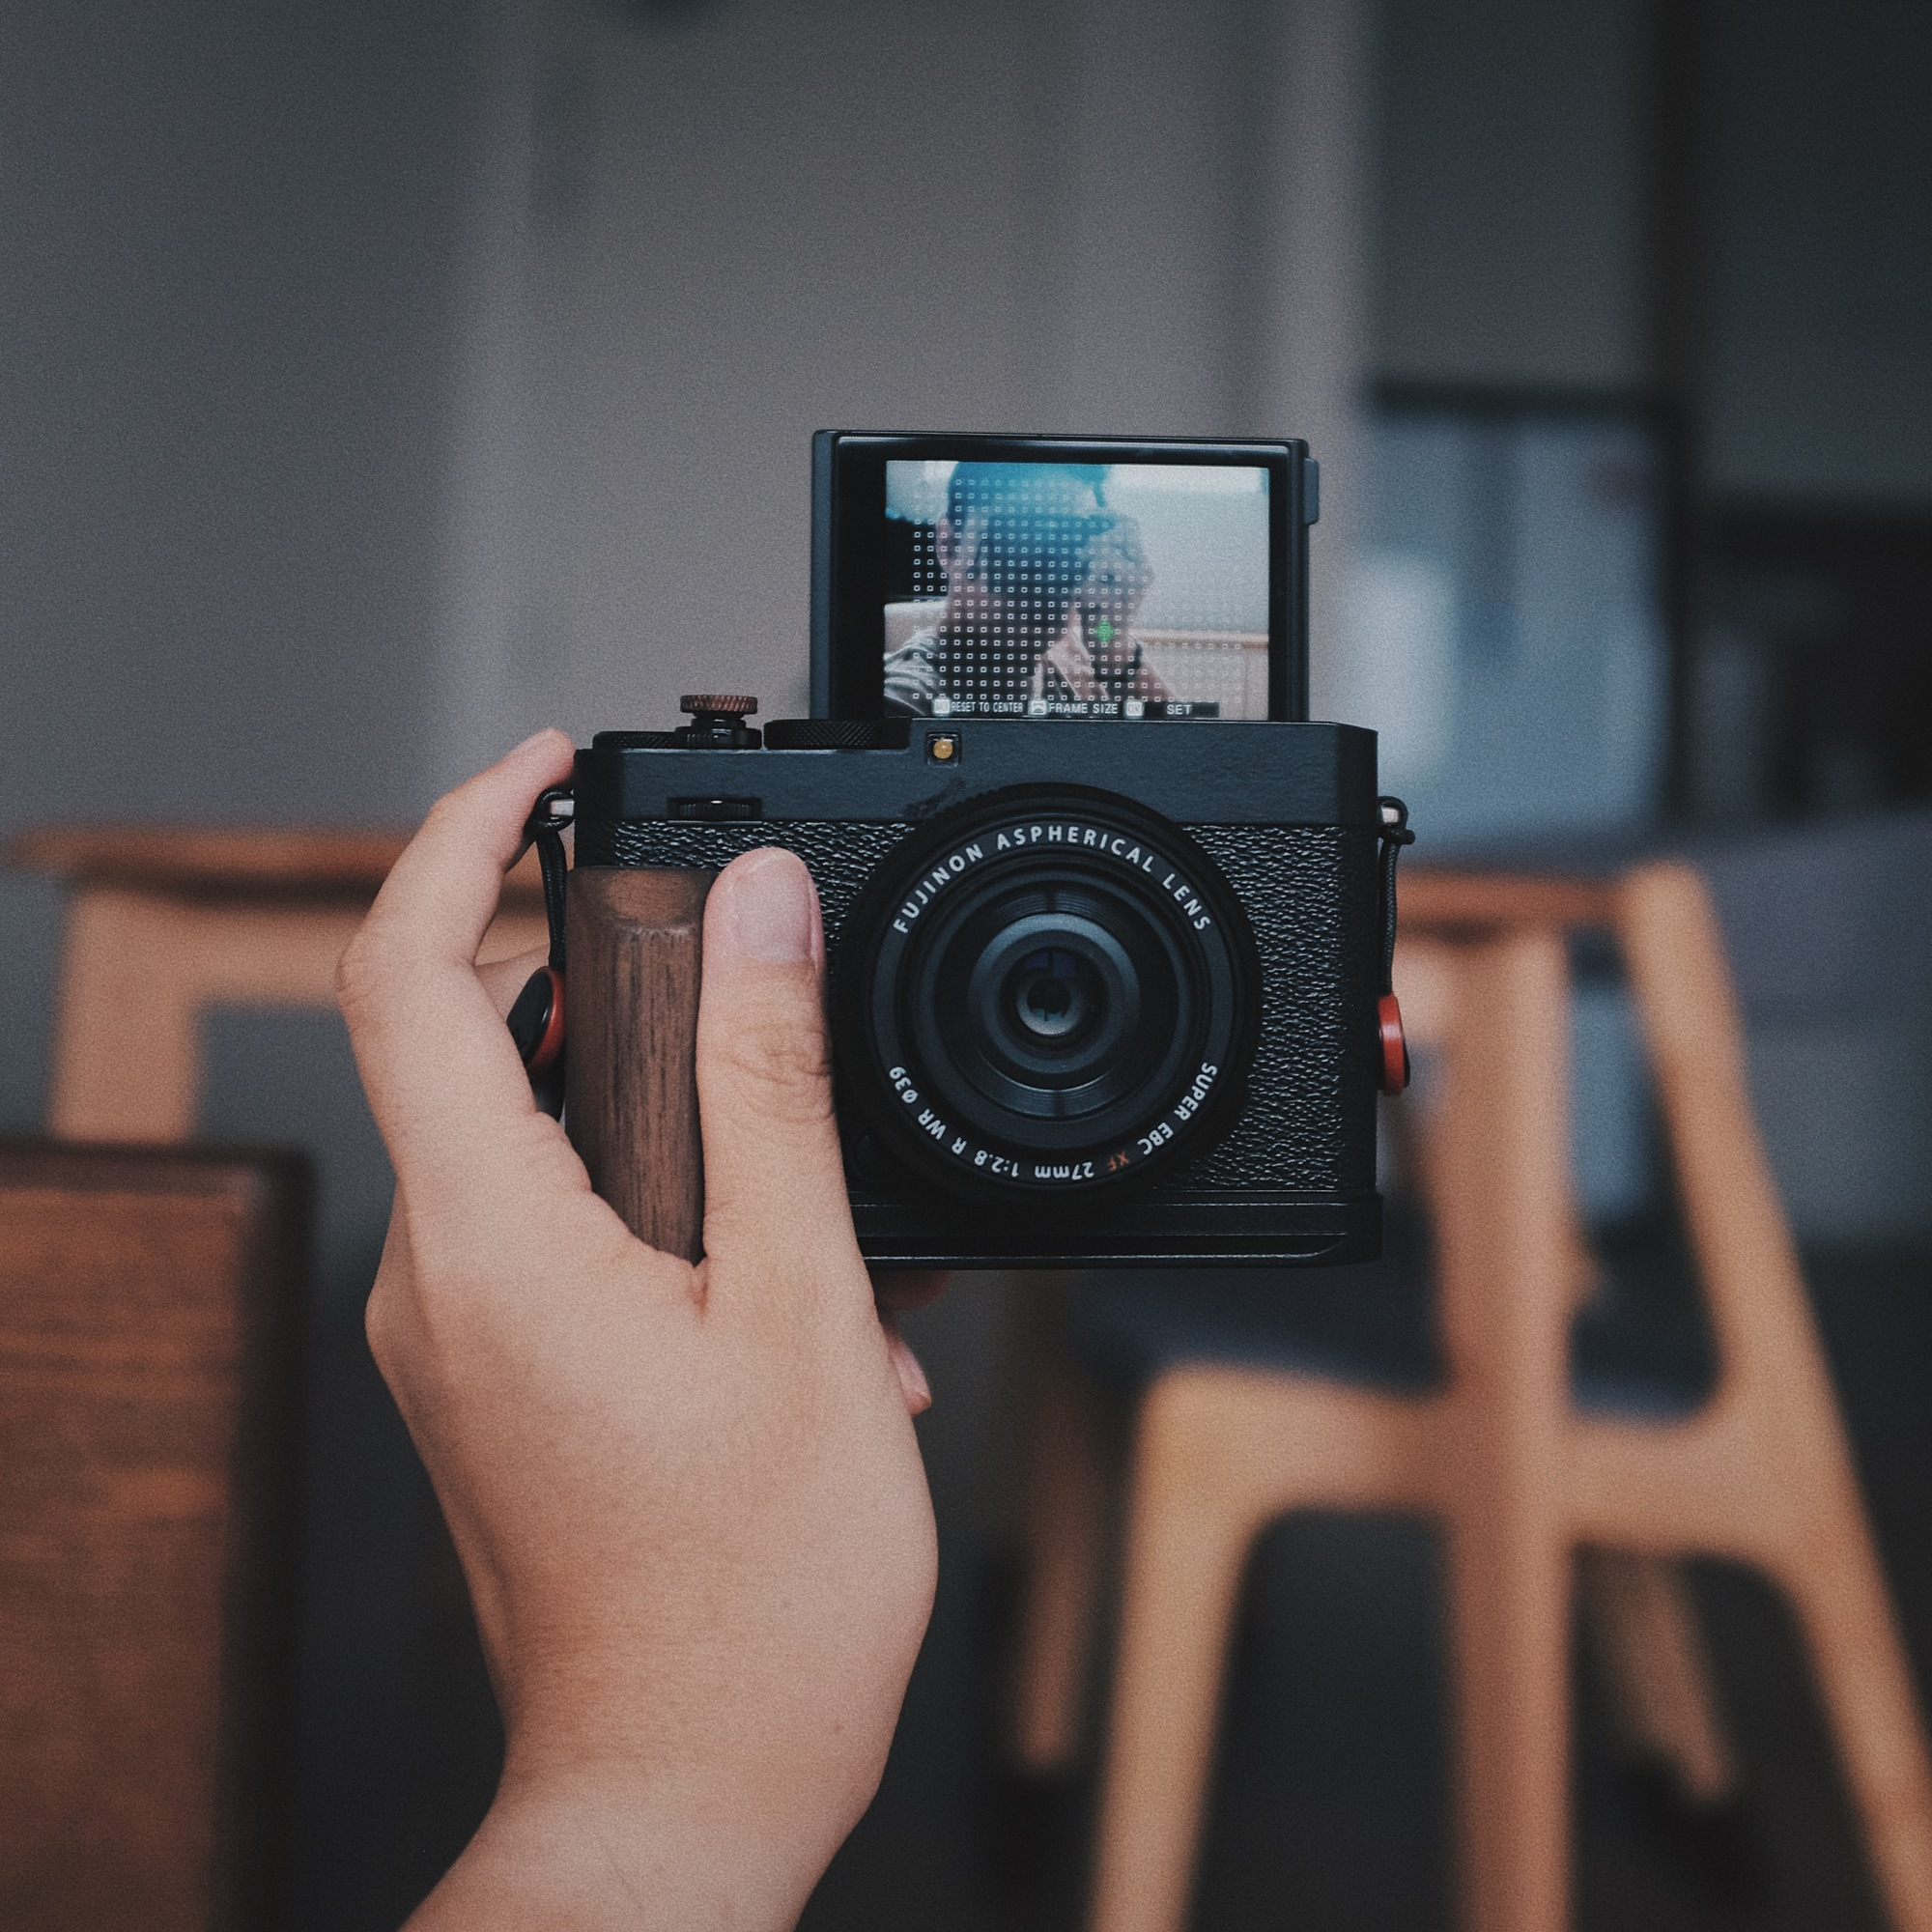
\includegraphics[width=\linewidth]{\envfinaldir/coverpic-prod.jpg}\par
            % \vskip 30pt
            \vfill

            \normalsize\rmfamily\scshape
            \copyright{} The Web Digest Project \hfill\large \envdatestr
        \end{center}
    \end{titlepage}
    % \restoregeometry
}
\newcommand{\simplehref}[1]{%
    \textcolor{blue!80!green}{\href{#1}{#1}}%
}
\renewcommand{\contentsname}{\center\Huge\sffamily\bfseries Contents\par\vskip 20pt}
\newcounter{ipartcounter}
\setcounter{ipartcounter}{0}
\newcommand{\ipart}[1]{
    % \vskip 20pt
    \clearpage
    \stepcounter{ipartcounter}
    \phantomsection
    \addcontentsline{toc}{chapter}{#1}
    % \begin{center}
    %     \Huge
    %     \sffamily\bfseries
    %     #1
    % \end{center}
    % \vskip 20pt plus 7pt
}
\newcounter{ichaptercounter}
\setcounter{ichaptercounter}{0}
\newcommand{\ichapter}[1]{
    % \vskip 20pt
    \clearpage
    \stepcounter{ichaptercounter}
    \phantomsection
    \addcontentsline{toc}{section}{\numberline{\arabic{ichaptercounter}}#1}
    \begin{center}
        \Huge
        \sffamily\bfseries
        #1
    \end{center}
    \vskip 20pt plus 7pt
}
\newcommand{\entrytitlefont}[1]{\subsection*{\raggedright\Large\sffamily\bfseries#1}}
\newcommand{\entryitemGeneric}[2]{
    % argv: title, url
    \parbox{\linewidth}{
        \entrytitlefont{#1}\par\vskip 5pt
        \footnotesize\ttfamily\mdseries
        \simplehref{#2}
    }\vskip 11pt plus 11pt minus 1pt
}
\newcommand{\entryitemGithub}[3]{
    % argv: title, url, desc
    \parbox{\linewidth}{
        \entrytitlefont{#1}\par\vskip 5pt
        \footnotesize\ttfamily\mdseries
        \simplehref{#2}\par\vskip 5pt
        \small\rmfamily\mdseries#3
    }\vskip 11pt plus 11pt minus 1pt
}
\newcommand{\entryitemAp}[3]{
    % argv: title, url, desc
    \parbox{\linewidth}{
        \entrytitlefont{#1}\par\vskip 5pt
        \footnotesize\ttfamily\mdseries
        \simplehref{#2}\par\vskip 5pt
        \small\rmfamily\mdseries#3
    }\vskip 11pt plus 11pt minus 1pt
}
\newcommand{\entryitemHackernews}[3]{
    % argv: title, hnurl, rawurl
    % \parbox{\linewidth}{
    %     \entrytitlefont{#1}\par\vskip 5pt
    %     \footnotesize\ttfamily\mdseries
    %     \simplehref{#3}\par
    %     \textcolor{black!50}{\href{#2}{#2}}
    % }\vskip 11pt plus 11pt minus 1pt
    \begin{minipage}{\linewidth}
            \entrytitlefont{#1}\par\vskip 5pt
            \footnotesize\ttfamily\mdseries
            \simplehref{#3}\par
            \textcolor{black!50}{\href{#2}{#2}}
    \end{minipage}\par\vskip 11pt plus 11pt minus 1pt
}







\begin{document}

\makeheader

\tableofcontents\clearpage




\ipart{Developers}
\ichapter{Hacker News}
\entryitemTwoLinks{A postmortem of three recent issues}{https://news.ycombinator.com/item?id=45281139}{https://www.anthropic.com/engineering/a-postmortem-of-three-recent-issues}

\entryitemTwoLinks{Famous cognitive psychology experiments that failed to replicate}{https://news.ycombinator.com/item?id=45279898}{https://buttondown.com/aethermug/archive/aether-mug-famous-cognitive-psychology/}

\entryitemTwoLinks{Optimizing ClickHouse for Intel's 280 core processors}{https://news.ycombinator.com/item?id=45279792}{https://clickhouse.com/blog/optimizing-clickhouse-intel-high-core-count-cpu}

\entryitemTwoLinks{WASM 3.0 Completed}{https://news.ycombinator.com/item?id=45279384}{https://webassembly.org/news/2025-09-17-wasm-3.0/}

\entryitemTwoLinks{DeepMind and OpenAI win gold at ICPC}{https://news.ycombinator.com/item?id=45279357}{https://codeforces.com/blog/entry/146536}

\entryitemTwoLinks{Anthropic irks White House with limits on models' use}{https://news.ycombinator.com/item?id=45279143}{https://www.semafor.com/article/09/17/2025/anthropic-irks-white-house-with-limits-on-models-uswhite-house-with-limits-on-models-use}

\entryitemTwoLinks{DeepSeek writes less secure code for groups China disfavors?}{https://news.ycombinator.com/item?id=45278740}{https://www.washingtonpost.com/technology/2025/09/16/deepseek-ai-security/}

\entryitemTwoLinks{Depression reduces capacity to learn to actively avoid aversive events}{https://news.ycombinator.com/item?id=45278686}{https://www.eneuro.org/content/12/9/ENEURO.0034-25.2025}

\entryitemTwoLinks{Tinycolor supply chain attack post-mortem}{https://news.ycombinator.com/item?id=45278657}{https://sigh.dev/posts/ctrl-tinycolor-post-mortem/}

\entryitemTwoLinks{Ton Roosendaal to step down as Blender chairman and CEO}{https://news.ycombinator.com/item?id=45278279}{https://www.cgchannel.com/2025/09/ton-roosendaal-to-step-down-as-blender-chairman-and-ceo/}

\entryitemTwoLinks{Not Buying American Anymore}{https://news.ycombinator.com/item?id=45277346}{https://xd1.dev/2025/09/not-buying-american-anymore}

\entryitemTwoLinks{How to motivate yourself to do a thing you don't want to do}{https://news.ycombinator.com/item?id=45276987}{https://ashleyjanssen.com/how-to-motivate-yourself-to-do-a-thing-you-dont-want-to-do/}

\entryitemTwoLinks{YouTube addresses lower view counts which seem to be caused by ad blockers}{https://news.ycombinator.com/item?id=45276262}{https://9to5google.com/2025/09/16/youtube-lower-view-counts-ad-blockers/}

\entryitemTwoLinks{UUIDv47: Store UUIDv7 in DB, emit UUIDv4 outside (SipHash-masked timestamp)}{https://news.ycombinator.com/item?id=45275973}{https://github.com/stateless-me/uuidv47}

\entryitemTwoLinks{Firefox 143 for Android to introduce DoH}{https://news.ycombinator.com/item?id=45275444}{https://blog.mozilla.org/en/firefox/dns-android/}

\entryitemTwoLinks{Bringing fully autonomous rides to Nashville, in partnership with Lyft}{https://news.ycombinator.com/item?id=45275415}{https://waymo.com/blog/2025/09/waymo-is-coming-to-nashville-in-partnership-with-lyft}

\entryitemTwoLinks{Tau² benchmark: How a prompt rewrite boosted GPT-5-mini by 22\%}{https://news.ycombinator.com/item?id=45275354}{https://quesma.com/blog/tau2-benchmark-improving-results-smaller-models/}

\entryitemTwoLinks{Procedural Island Generation (III)}{https://news.ycombinator.com/item?id=45275049}{https://brashandplucky.com/2025/09/17/procedural-island-generation-iii.html}

\entryitemTwoLinks{Apple Photos app corrupts images}{https://news.ycombinator.com/item?id=45274277}{https://tenderlovemaking.com/2025/09/17/apple-photos-app-corrupts-images/}

\entryitemTwoLinks{Determination of the fifth Busy Beaver value}{https://news.ycombinator.com/item?id=45273999}{https://arxiv.org/abs/2509.12337}\ichapter{Phoronix}
\entryitemGeneric{\hskip 0pt{}AMD "GFX1251" Target Added To LLVM As Latest RDNA 4.5 APU}{https://www.phoronix.com/news/AMD-GFX1251-LLVM-Target}

\entryitemGeneric{\hskip 0pt{}OpenJDK 25 \& GraalVM 25 Released With 32-bit x86 Support Removed}{https://www.phoronix.com/news/OpenJDK-Java-25-GraalVM-25}

\entryitemGeneric{\hskip 0pt{}AMD Hardware Would Ideally Be Supported By ROCm For ~10 Years}{https://www.phoronix.com/news/AMD-ROCm-Hardware-Length}

\entryitemGeneric{\hskip 0pt{}GNOME 49 Officially Released With Wayland Improvements, Showtime As Video Player}{https://www.phoronix.com/news/GNOME-49-Released}

\entryitemGeneric{\hskip 0pt{}Latest Open-Source AMD Improvements Allowing For Better Llama.cpp AI Performance Against Windows 11}{https://www.phoronix.com/review/llama-cpp-windows-linux}

\entryitemGeneric{\hskip 0pt{}A Quick Look At The AMD Instinct MI355X With ROCm 7.0}{https://www.phoronix.com/news/AMD-Instinct-MI355X-ROCm-7.0}

\entryitemGeneric{\hskip 0pt{}systemd 258 Released With systemd-factory-reset \& Other New Tools}{https://www.phoronix.com/news/systemd-258}

\entryitemGeneric{\hskip 0pt{}Microsoft Rolls Out A Linux 6.12 LTS Option For Azure Linux}{https://www.phoronix.com/news/Azure-Linux-3.0.20250910}

\entryitemGeneric{\hskip 0pt{}Linux 6.18 To Add Detection For FreeBSD's Bhyve Hypervisor}{https://www.phoronix.com/news/Linux-6.18-Detect-Bhyve}


\ipart{Developers~~~~(zh-Hans)}
\ichapter{Solidot}
\entryitemGeneric{\hskip 0pt{}迪士尼华纳等起诉中国 AI 公司侵犯版权}{https://www.solidot.org/story?sid=82343}

\entryitemGeneric{\hskip 0pt{}气候暖化会让土壤释放出更多碳}{https://www.solidot.org/story?sid=82342}

\entryitemGeneric{\hskip 0pt{}字节跳动阿里巴巴等公司被要求停止购买英伟达 AI 芯片}{https://www.solidot.org/story?sid=82341}

\entryitemGeneric{\hskip 0pt{}NPM 再次发现供应链攻击 }{https://www.solidot.org/story?sid=82340}

\entryitemGeneric{\hskip 0pt{}M87*黑洞图像显示其偏振方向发生翻转}{https://www.solidot.org/story?sid=82339}

\entryitemGeneric{\hskip 0pt{}Firefox 143.0 释出}{https://www.solidot.org/story?sid=82338}

\entryitemGeneric{\hskip 0pt{}白垩纪兽脚类恐龙奔跑时速能达到 45 公里}{https://www.solidot.org/story?sid=82337}

\entryitemGeneric{\hskip 0pt{}AMD 终止自己的 AMDVLK 开源驱动项目,拥抱社区项目 Mesa RADV}{https://www.solidot.org/story?sid=82336}

\entryitemGeneric{\hskip 0pt{}苹果为 10 年前的 iPhone 6 释出安全更新}{https://www.solidot.org/story?sid=82335}

\entryitemGeneric{\hskip 0pt{}甲骨文、银湖和 Andreessen Horowitz 组成的财团将收购 TikTok 美国业务 }{https://www.solidot.org/story?sid=82333}

\entryitemGeneric{\hskip 0pt{}用户如何使用 ChatGPT?}{https://www.solidot.org/story?sid=82332}

\entryitemGeneric{\hskip 0pt{}TRAPPIST-1e 可能是至今发现的最类似地球的行星}{https://www.solidot.org/story?sid=82331}

\entryitemGeneric{\hskip 0pt{}Java 25 释出}{https://www.solidot.org/story?sid=82330}

\entryitemGeneric{\hskip 0pt{}韦伯捕捉到长 8 光年的原恒星喷流}{https://www.solidot.org/story?sid=82329}

\entryitemGeneric{\hskip 0pt{}Varnish 8.0.0 释出,因 IP 争议将改名}{https://www.solidot.org/story?sid=82328}

\entryitemGeneric{\hskip 0pt{}蚁后被发现产下了两个不同物种的蚂蚁}{https://www.solidot.org/story?sid=82326}

\entryitemGeneric{\hskip 0pt{}AOMedia 联盟将于年底发布 AV2 编解码器}{https://www.solidot.org/story?sid=82325}

\entryitemGeneric{\hskip 0pt{}Godot 4.5 释出}{https://www.solidot.org/story?sid=82324}

\entryitemGeneric{\hskip 0pt{}Microsoft 365 应用将从下个月起强制安装 Copilot Chat}{https://www.solidot.org/story?sid=82323}

\entryitemGeneric{\hskip 0pt{}Google 改变了 Android 的安全更新模式}{https://www.solidot.org/story?sid=82322}\ichapter{V2EX}
\entryitemGeneric{\hskip 0pt{}[分享发现] 按照目前这个退休年龄,要是哪天我儿子进了和我同样的公司,职级还比我高,感觉还有点怪怪的}{https://www.v2ex.com/t/1160067}

\entryitemGeneric{\hskip 0pt{}[Steam] Steam deck 原生桌面有办法运行 exe 小游戏吗?}{https://www.v2ex.com/t/1160066}

\entryitemGeneric{\hskip 0pt{}[分享创造] [分享创造] ICOAPEX | 一键生成专属商标与全格式图标 - 免费送激活码}{https://www.v2ex.com/t/1160065}

\entryitemGeneric{\hskip 0pt{}[跑步] 报名了波士顿马拉松}{https://www.v2ex.com/t/1160064}

\entryitemGeneric{\hskip 0pt{}[C\#] .NET 换新的异步编程模型了,性能很强}{https://www.v2ex.com/t/1160063}

\entryitemGeneric{\hskip 0pt{}[Apple] Apple Notes 实现 Blog 自动同步,并且支持文章加密。}{https://www.v2ex.com/t/1160062}

\entryitemGeneric{\hskip 0pt{}[iPhone] iOS 26 Safari 书签浏览的问题}{https://www.v2ex.com/t/1160061}

\entryitemGeneric{\hskip 0pt{}[问与答] 哔哩哔哩如何将``动态''里的 UP 进行分组}{https://www.v2ex.com/t/1160060}

\entryitemGeneric{\hskip 0pt{}[问与答] 博朗 5 系续航崩了,是不是该换了}{https://www.v2ex.com/t/1160059}

\entryitemGeneric{\hskip 0pt{}[香港] 2025-09-12 香港银行开户经历分享}{https://www.v2ex.com/t/1160058}

\entryitemGeneric{\hskip 0pt{}[推广] Marble 模型今天发布,只需一张图片,就能生成持久存在的 3D 世界}{https://www.v2ex.com/t/1160057}

\entryitemGeneric{\hskip 0pt{}[音乐] Spotify 太会推荐了吧}{https://www.v2ex.com/t/1160054}

\entryitemGeneric{\hskip 0pt{}[问与答] 为什么我在一个 App 搜过的东西,会在另一个 App 出现推荐?能不能用``噪声''来反追踪?}{https://www.v2ex.com/t/1160053}

\entryitemGeneric{\hskip 0pt{}[分享发现] 18+的网页游戏可以过 Adsense 吗?}{https://www.v2ex.com/t/1160051}

\entryitemGeneric{\hskip 0pt{}[问与答] 信用卡谷歌云和亚马逊云认证问题}{https://www.v2ex.com/t/1160050}

\entryitemGeneric{\hskip 0pt{}[随想] 也观隔壁买车推荐有感,人心中的成见是一座大山。}{https://www.v2ex.com/t/1160049}

\entryitemGeneric{\hskip 0pt{}[ WATCH] 哪些三合一充电器可以给港版 apple watch s10/s11 快充?}{https://www.v2ex.com/t/1160048}

\entryitemGeneric{\hskip 0pt{}[Solana] 不是说 v 币这里没夹子的吗?}{https://www.v2ex.com/t/1160047}

\entryitemGeneric{\hskip 0pt{}[Solana] 手上有几个独立的节点, 可以做点什么有意思的事情吗?}{https://www.v2ex.com/t/1160046}

\entryitemGeneric{\hskip 0pt{}[求职] 「全职自由 UI 设计师」十年+经验 - 寻求远程兼职机会}{https://www.v2ex.com/t/1160045}

\entryitemGeneric{\hskip 0pt{}[服务器] 绿云 70 刀 3 年软银补货 7 台,手慢无!}{https://www.v2ex.com/t/1160044}

\entryitemGeneric{\hskip 0pt{}[问与答] 有做过近视手术的朋友进来分享下体验吧}{https://www.v2ex.com/t/1160043}

\entryitemGeneric{\hskip 0pt{}[香港] 香港 cmhk 手机卡能在内地保号吗}{https://www.v2ex.com/t/1160042}

\entryitemGeneric{\hskip 0pt{}[macOS] 更新到 macOS Tahoe 26.0 后, Aldente 无法工作}{https://www.v2ex.com/t/1160041}

\entryitemGeneric{\hskip 0pt{}[问与答] 极摩客 k5 7735hs 玩机方案求教}{https://www.v2ex.com/t/1160040}

\entryitemGeneric{\hskip 0pt{}[分享发现] 国内大数据下真就一点隐私都没有}{https://www.v2ex.com/t/1160039}

\entryitemGeneric{\hskip 0pt{}[Apple] 看测试,苹果新的 40w 单口 PD3.2 充电头严重虚标啊}{https://www.v2ex.com/t/1160037}

\entryitemGeneric{\hskip 0pt{}[推广] 分享一个企业级 AI Gateway 支持各种大模型订阅}{https://www.v2ex.com/t/1160036}

\entryitemGeneric{\hskip 0pt{}[OpenAI] codex-cli 用着非常慢非常慢}{https://www.v2ex.com/t/1160035}

\entryitemGeneric{\hskip 0pt{}[问与答] 送礼求助}{https://www.v2ex.com/t/1160034}

\entryitemGeneric{\hskip 0pt{}[Apple] iPadOS26 卡死,无法关机}{https://www.v2ex.com/t/1160033}

\entryitemGeneric{\hskip 0pt{}[macOS] macos26 有什么远程控制的推荐?}{https://www.v2ex.com/t/1160032}

\entryitemGeneric{\hskip 0pt{}[酷工作] 招聘远程 web3 开发人员,月 base 3w-5w, 13 薪}{https://www.v2ex.com/t/1160030}

\entryitemGeneric{\hskip 0pt{}[Solana] 币安抢空投目前发现最好用的工具}{https://www.v2ex.com/t/1160028}

\entryitemGeneric{\hskip 0pt{}[Steam] SreamOS 系统下如何通过命令行完整卸载一款软件?}{https://www.v2ex.com/t/1160027}

\entryitemGeneric{\hskip 0pt{}[投资] 有两融需求的看过来!拼单开户拿更低利率~}{https://www.v2ex.com/t/1160026}

\entryitemGeneric{\hskip 0pt{}[Apple] safari26 默认缩放问题}{https://www.v2ex.com/t/1160025}

\entryitemGeneric{\hskip 0pt{}[分享创造] 使用睡前消息音色进行的二次创作}{https://www.v2ex.com/t/1160024}

\entryitemGeneric{\hskip 0pt{}[问与答] 一直用 altstore 多开微信,升级 ios26 警告我准用外挂了}{https://www.v2ex.com/t/1160023}

\entryitemGeneric{\hskip 0pt{}[DJI] 哪位有 VelociDrone}{https://www.v2ex.com/t/1160021}

\entryitemGeneric{\hskip 0pt{}[分享创造] 自己开发的工具网站分享给大家,应该还算美观}{https://www.v2ex.com/t/1160020}

\entryitemGeneric{\hskip 0pt{}[Apple] 传 MacBook Pro 将于 2027 年支持触摸屏!}{https://www.v2ex.com/t/1160019}

\entryitemGeneric{\hskip 0pt{}[iPhone] 分享一张 esim}{https://www.v2ex.com/t/1160018}

\entryitemGeneric{\hskip 0pt{}[程序员] 新书上架(抽奖)- 《深入高可用系统原理与设计》}{https://www.v2ex.com/t/1160016}

\entryitemGeneric{\hskip 0pt{}[Solana] 终于进前一百了🎉}{https://www.v2ex.com/t/1160015}

\entryitemGeneric{\hskip 0pt{}[Windows] 为什么网络慢,电脑就会变慢,这样的设计合理吗?}{https://www.v2ex.com/t/1160014}

\entryitemGeneric{\hskip 0pt{}[程序员] Augment 已经没有免费帐户了}{https://www.v2ex.com/t/1160013}

\entryitemGeneric{\hskip 0pt{}[投资] 哎,税务局打电话给公司财务,让我去税务局说境外所得的事}{https://www.v2ex.com/t/1160012}

\entryitemGeneric{\hskip 0pt{}[汽车] 国内特斯拉如何装 Spotify}{https://www.v2ex.com/t/1160011}

\entryitemGeneric{\hskip 0pt{}[Apple] mac studio 是可以不激活使用的吗?}{https://www.v2ex.com/t/1160010}


\ipart{Generic News}







\clearpage
\leavevmode\vfill
\footnotesize

Copyright \copyright{} 2023-2025 Neruthes and other contributors.

This document is published with CC BY-NC-ND 4.0 license.

The entries listed in this newsletter may be copyrighted by their respective creators.

This newsletter is generated by the Web Digest project.

The newsletters are also delivered via Telegram channel \CJKunderline{\href{https://t.me/webdigestchannel}{https://t.me/webdigestchannel}}.\\
RSS feed is available at \CJKunderline{\href{https://webdigest.pages.dev/rss.xml}{https://webdigest.pages.dev/rss.xml}}.

This newsletter is available in PDF at
\CJKunderline{\href{https://webdigest.pages.dev/}{https://webdigest.pages.dev/}}.

The source code being used to generate this newsletter is available at\\
\CJKunderline{\href{https://github.com/neruthes/webdigest}{https://github.com/neruthes/webdigest}}.

This newsletter is also available in
\CJKunderline{\href{http://webdigest.pages.dev/readhtml/\envyear/WebDigest-20250918.html}{HTML}} and
\CJKunderline{\href{https://github.com/neruthes/webdigest/blob/master/markdown/\envyear/WebDigest-20250918.md}{Markdown}}.


\coverpic{https://unsplash.com/photos/a-vintage-camera-rests-on-a-wooden-surface-4vIfHinwrvM}{Eduardo Gorghetto}


\end{document}
